\chapter{Cuestionario de interés inicial en la aplicación}\label{Anexo:CuestionarioInicial}
\section{Introducción}

A principios de marzo de este año 2025, durante mi participación en el programa Santander X Explorer, realicé una encuesta con el objetivo de recopilar opiniones de posibles usuarios sobre una aplicación diseñada para optimizar la gestión y coordinación en casos de desapariciones. Esta herramienta busca conectar a fuerzas de seguridad, grupos de rescate, voluntarios y población general, fomentando una participación ciudadana segura y eficiente.

El propósito de la encuesta era identificar las necesidades, expectativas y disposición de uso por parte de los potenciales usuarios, con el fin de diseñar una solución realmente útil y adaptada a sus preferencias. La encuesta sigue actualmente activa en el enlace \url{https://forms.gle/mvGdgDk62KTJWKVL9}, por si fuera de su interés participar.

\section{Resultados}
Se encuestaron un total de 115 personas, distribuidas entre población civil (105), grupos voluntarios (7) y personal de Fuerzas y Cuerpos de Seguridad del Estado (FFCCS) (3). La distribución geográfica y por edades puede consultarse en las siguientes figuras:


%\figura{0.9}{img/RespuestasEncuesta/Edad.png }{Distribución de respuestas a la encuesta por edad. \textit{Fuente propia.}}{Encuesta:Edad}{keepaspectratio}

%\figura{0.9}{img/RespuestasEncuesta/distGruposRepresentativos.png }{Distribución de respuestas a la encuesta por grupos. \textit{Fuente propia.}}{Encuesta:Pais}{keepaspectratio}

%\figura{0.9}{img/RespuestasEncuesta/Pais.png }{Distribución de respuestas a la encuesta por países. \textit{Fuente propia.}}{Encuesta_distGrupos}{keepaspectratio}

\begin{figure}[h!]
\centering
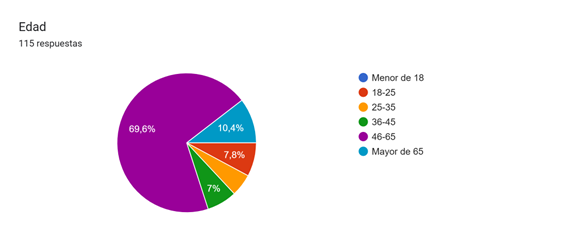
\includegraphics[width=0.9\textwidth, keepaspectratio]{img/RespuestasEncuesta/Edad.png}
\caption{Distribución de respuestas a la encuesta por edad. \textit{Fuente propia.}}
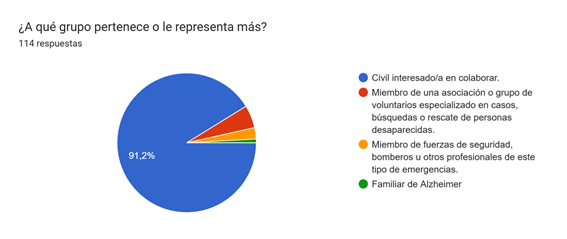
\includegraphics[width=0.9\textwidth, keepaspectratio]{img/RespuestasEncuesta/distGruposRepresentativos.png}
\caption{Distribución de respuestas a la encuesta por grupos. \textit{Fuente propia.}}
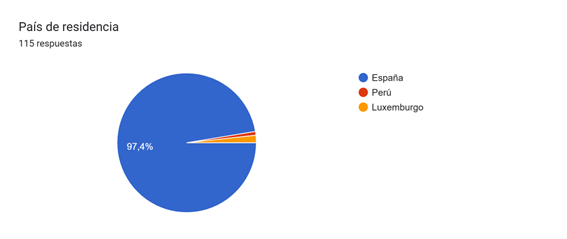
\includegraphics[width=0.9\textwidth, keepaspectratio]{img/RespuestasEncuesta/Pais.png}
\caption{Distribución de respuestas a la encuesta por países. \textit{Fuente propia.}}
\caption{Distribuciones de respuestas de la encuesta. \textit{Fuente propia.}}
\label{fig:encuesta}
\end{figure}


\vspace{3cm}

\subsubsection{Civiles interesados en colaborar}

La mayoría de los encuestados civiles no había pertenecido previamente a grupos relacionados con personas desaparecidas. Sin embargo, un porcentaje significativo había colaborado alguna vez en la búsqueda de personas desaparecidas, principalmente compartiendo avisos en redes sociales y aplicaciones de mensajería. Algunos también participaron activamente en búsquedas sobre el terreno como voluntarios.

\begin{figure}[h!]
\centering
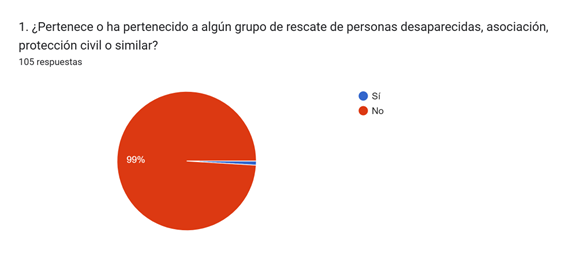
\includegraphics[width=0.9\textwidth, keepaspectratio]{img/RespuestasEncuesta/C_P1.png}
\caption{Respuesta a la pregunta 1  de civiles de la encuesta. \textit{Fuente propia.}}
\label{Encuesta_C_P1}
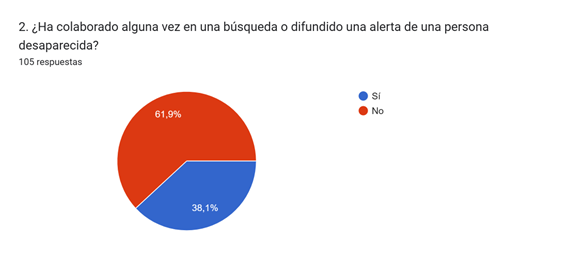
\includegraphics[width=0.9\textwidth, keepaspectratio]{img/RespuestasEncuesta/C_P2.png}
\caption{Respuesta a la pregunta 2  de civiles de la encuesta. \textit{Fuente propia.}}
\label{Encuesta_C_P2}
\end{figure}

%\figura{0.9}{img/RespuestasEncuesta/C_P1.png}{Respuesta a la pregunta 1  de civiles de la encuesta. \textit{Fuente propia.}}{Encuesta_C_P1}{keepaspectratio}

%\figura{0.95}{img/RespuestasEncuesta/C_P2.png}{Respuesta a la pregunta 2  de civiles de la encuesta. \textit{Fuente propia.}}{Encuesta_C_P2}{keepaspectratio}

Casi la mitad de los encuestados civiles afirmaron que se descargarían una aplicación que enviara alertas de personas desaparecidas en su zona. Un 46\% adicional manifestó dudas. La motivación más frecuente para descargar la app era la voluntad de ayudar y colaborar.

\begin{figure}[h!]
    \centering
    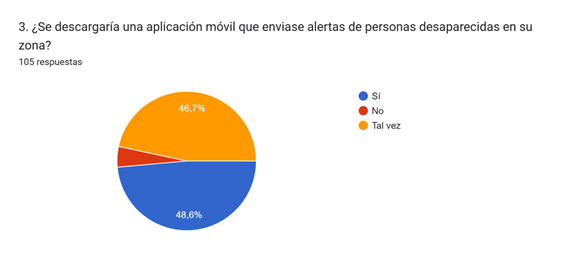
\includegraphics[width=0.9\linewidth]{img/RespuestasEncuesta/C_P3.png}
    \caption{Respuesta a la pregunta 3  de civiles de la encuesta. \textit{Fuente propia.}}
    \label{Encuesta_C_P3}
\end{figure}
%\figura{1}{img/RespuestasEncuesta/C_P3.png}{Respuesta a la pregunta 3  de civiles de la encuesta. \textit{Fuente propia.}}{Encuesta_C_P3}{keepaspectratio}

\vspace{3cm}

La mayoría también expresó disposición para colaborar voluntariamente en búsquedas activas.

\begin{figure}[h!]
\centering
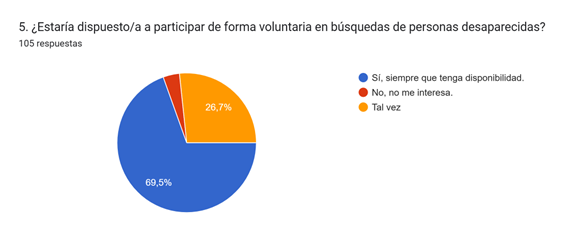
\includegraphics[width=0.85\textwidth, keepaspectratio]{img/RespuestasEncuesta/C_P5.png}
\caption{Respuesta a la pregunta 5  de civiles de la encuesta. \textit{Fuente propia.}}
\label{Encuesta_C_P5}
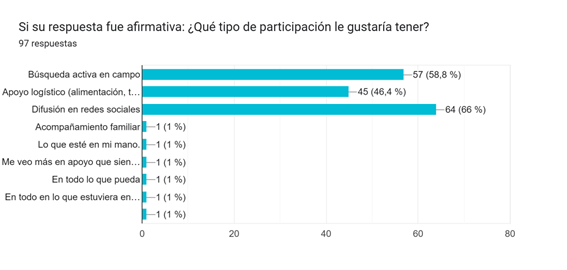
\includegraphics[width=0.85\textwidth, keepaspectratio]{img/RespuestasEncuesta/C_P5_2.png}
\caption{Respuesta a la segunda parte de la pregunta 5 a civiles de la encuesta. \textit{Fuente propia.}}
\label{Encuesta_C_P5_2}
\end{figure}

%\figura{0.85}{img/RespuestasEncuesta/C_P5.png}{Respuesta a la pregunta 5  de civiles de la encuesta. \textit{Fuente propia.}}{Encuesta_C_P5}{keepaspectratio}
%\figura{0.9}{img/RespuestasEncuesta/C_P5_2.png}{Respuesta a la segunda parte de la pregunta 5 a civiles de la encuesta. \textit{Fuente propia.}}{Encuesta_C_P5_2}{keepaspectratio}

En cuanto a funcionalidades, la más valorada fue la posibilidad de recibir alertas de desapariciones en su zona.

\begin{figure}[h!]
    \centering
    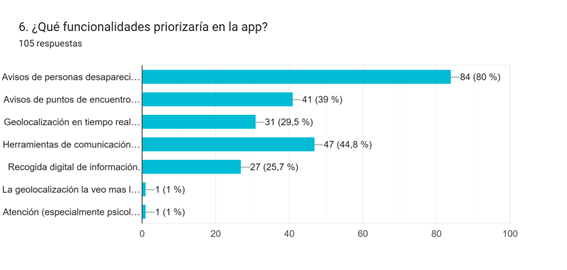
\includegraphics[width=0.85\linewidth]{img/RespuestasEncuesta/C_P6.png}
    \caption{Respuesta a la pregunta 6  de civiles de la encuesta. \textit{Fuente propia.}}
    \label{Encuesta_C_P6}
\end{figure}
%\figura{0.95}{img/RespuestasEncuesta/C_P6.png}{Respuesta a la pregunta 6  de civiles de la encuesta. \textit{Fuente propia.}}{Encuesta_C_P6}{keepaspectratio}

\vspace{5cm}
\subsubsection{Respuestas de miembros de grupos relacionados con casos de personas desaparecidas}

Aunque la muestra fue reducida, se obtuvieron respuestas de diversos colectivos como distintos puestos de Protección Civil, grupos de rescate especializados y asociaciones vinculadas a enfermedades como el Alzheimer.

Las herramientas actualmente utilizadas incluyen documentos en papel, la aplicación Alerthor, mapas topográficos, grupos de WhatsApp y dispositivos GPS.

Todos los encuestados de este grupo manifestaron interés en utilizar una herramienta digital que facilite la coordinación y divulgación de búsquedas. La mayoría también valoró positivamente la posibilidad de conectar con otros grupos y voluntarios mediante una app.

\figura{0.9}{img/RespuestasEncuesta/G_P4.png}{Respuestas a la pregunta 4 de los grupos no pertenecientes a las FFCCS. \textit{Fuente propia.}}{Encuesta_G_P4}{keepaspectratio}

\figura{0.9}{img/RespuestasEncuesta/G_P5.png}{Respuestas a la pregunta 5 de los grupos no pertenecientes a las FFCCS. \textit{Fuente propia.}}{Encuesta_G_P5}{keepaspectratio}

\vspace{7cm}

Las funcionalidades más relevantes para este grupo fueron:
\begin{itemize}
	\item Geolocalización en tiempo real de los participantes.
	\item Recepción de avisos de desapariciones.
	\item Control de áreas ya cubiertas.
	\item Establecimiento de puntos de control durante las búsquedas.
	\item Recogida digital de la información.
	\item Gestión de tareas logísticas desde un único lugar.
\end{itemize}

También se valoraron, aunque en menor medida, funcionalidades como la predicción de localización de la persona desaparecida y obtención del listado completo de participantes en la búsqueda.

\figura{0.95}{img/RespuestasEncuesta/G_P6.png}{Respuestas a la pregunta 6  de los grupos no pertenecientes a las FFCCS. \textit{Fuente propia.}}{Encuesta_G_P6}{keepaspectratio}

Desde estos colectivos se subrayó la importancia de que la aplicación forme parte del sistema oficial de coordinación, gestionado por el puesto de mando, y utilizada exclusivamente por los intervinientes, para evitar el intrusismo y garantizar la profesionalidad en estos dispositivos.


\subsubsection{Miembros de fuerzas de seguridad, bomberos u otros profesionales}

Aunque la participación de personal de FFCCS fue limitada, se recibieron respuestas de policías nacionales y miembros de las fuerzas armadas.

Las herramientas principales utilizadas incluyen bases de datos policiales. Todos los encuestados consideraron útil una aplicación que automatice los avisos y facilite la coordinación entre grupos de rescate y civiles.

\vspace{3cm}

Las funcionalidades más valoradas fueron:
\begin{itemize}
	\item Herramientas de comunicación entre voluntarios y grupos de rescate.
	\item Recogida digital de la información.
	\item Avisos de desapariciones com opción de difusión en redes sociales.
\end{itemize}

\figura{1}{img/RespuestasEncuesta/FFCCS_P4.png}{Respuestas a la pregunta 4  de los grupos pertenecientes a las FFCCS. \textit{Fuente propia.}}{Encuesta_FFCCS_P4}{keepaspectratio}

\figura{1}{img/RespuestasEncuesta/FFCCS_P5.png}{Respuestas a la pregunta 5  de los grupos pertenecientes a las FFCCS. \textit{Fuente propia.}}{Encuesta_FFCCS_P5}{keepaspectratio}


